\documentclass[10pt,a4paper]{article}
\usepackage[T1]{fontenc}
\usepackage{lmodern,amsmath,amssymb,booktabs,array,xcolor,microtype}
\usepackage[margin=16mm,top=14mm,bottom=16mm]{geometry}
\usepackage{fancyhdr,tikz,graphicx}
\usepackage[hidelinks]{hyperref}
\definecolor{navy}{HTML}{17324D}
\definecolor{teal}{HTML}{176E78}
\definecolor{pale}{HTML}{EEF5F7}
\definecolor{muted}{HTML}{4B5963}
\definecolor{rulegray}{HTML}{CAD5DB}
\setlength{\parindent}{0pt}
\setlength{\parskip}{3pt}
\setlength{\abovedisplayskip}{4pt}
\setlength{\belowdisplayskip}{4pt}
\setlength{\abovedisplayshortskip}{3pt}
\setlength{\belowdisplayshortskip}{3pt}
\pagestyle{fancy}\fancyhf{}
\renewcommand{\headrulewidth}{0pt}
\fancyfoot[L]{\scriptsize\color{muted}QVDF-E \quad | \quad Arizona detector 141 worked example}
\fancyfoot[R]{\scriptsize\color{muted}\thepage\ / 7}
\newcommand{\method}[2]{\par\vspace{4pt}{\color{teal}\bfseries #1\quad #2}\par\vspace{1pt}}
\newcommand{\notebox}[1]{\par\vspace{4pt}\begingroup\setlength{\fboxsep}{7pt}\colorbox{pale}{\parbox{\dimexpr\linewidth-14pt\relax}{#1}}\endgroup\par}
\hypersetup{pdftitle={QVDF-E: Arizona detector 141 emission diagnostic},pdfauthor={Mohammad Abbasi},pdfsubject={Equations and verified average-weekday results}}
\definecolor{methodO}{HTML}{242B33}
\definecolor{methodS}{HTML}{2563EB}
\definecolor{methodR}{HTML}{7B3294}
\definecolor{methodM}{HTML}{168C69}
\definecolor{methodA}{HTML}{E69F00}\newcommand{\legendkey}[2]{{\scriptsize\textcolor{#1}{\rule[2pt]{10pt}{1.3pt}}\ #2}}
\begin{document}
\fontsize{9.3}{11.1}\selectfont
{\fontsize{19}{22}\selectfont\bfseries\color{navy}Five emission calculations}\par
{\color{muted}One whole episode, one pollutant. O, S, R, M and A identify the existing calculations.}

\textbf{Notation and units.} Bin $i$ has speed $v_i$ and count $d_i=q_i\Delta t$, with $\Delta t=1/12$ h.
$D=\sum_i d_i$; $L$ is link length; $C$ is hourly capacity; $T_f=L/v_f$.
$H$ denotes vehicle-hours, $P$ episode duration and $T$ per-vehicle travel time.
$r_0(v)$ is the zero-acceleration lookup rate in g/(veh\,h); $E$ is in grams. Counts and capacity use the same lane basis.

\textbf{Shared fitted quantities for R, M and A.}
\[
x=\frac{D}{C},\qquad \widehat P=\max(f_dx^n,x),\qquad
\widehat w_{\max}=T_f f_p\widehat P^{s},\qquad
\widehat{\bar w}=\theta\widehat w_{\max},\qquad
H_{\rm pred}=D(T_f+\widehat{\bar w}).
\]
$f_d,n,f_p,s,\theta$ are calibrated by directional corridor and period, with the existing sparse-period fallback.

\method{O}{Recorded-speed reference}
Assign each bin's counted vehicles the complete-link travel time $L/v_i$, then sum:
\[
H_i=d_i\frac{L}{v_i},\qquad H_{\rm obs}=\sum_i H_i,\qquad
\boxed{E_O=\sum_i H_i r_0(v_i).}
\]
The five-minute interval supplies the count; emission exposure is $L/v_i$, not five minutes.

\method{S}{Episode mean-speed estimate}
Use the count-weighted harmonic mean, preserving the reference's total vehicle-hours:
\[
\bar v_{\rm obs}=\frac{D}{\sum_i d_i/v_i}=\frac{DL}{H_{\rm obs}},\qquad
\boxed{E_S=H_{\rm obs}\,r_0(\bar v_{\rm obs}).}
\]

\method{R}{Reconstructed whole-link speeds}
For normalized entry time $u\in[0,1]$, define $w(u)=\widehat w_{\max}h(u)$ and
$v_R(u)=L/[T_f+w(u)]$. The symmetric profile is
\[
h(u)=\begin{cases}
[4u(1-u)]^a,&\theta\le 2/3,\quad \int_0^1h(u)\,du=\theta\ \text{determines }a,\\
1-|2u-1|^b,&\theta>2/3,\quad b=\theta/(1-\theta).
\end{cases}
\]
The entering-vehicle weight is $dN=D[1+(\widehat w_{\max}/\widehat P)h'(u)]\,du$. Thus
\[
\boxed{E_R=\int_0^1[T_f+w(u)]\,r_0\!\left(\frac{L}{T_f+w(u)}\right)\,dN.}
\]
The integral uses 384 quadrature points; $\int dN=D$ and $\int[T_f+w(u)]dN=H_{\rm pred}$.
These are trip-average speeds by entry time, not individual operating-speed trajectories.

\method{M}{Two-speed lookup}
Infer the queue speed from discharge and the triangular fundamental diagram:
\[
\widehat\mu=\frac{D}{\widehat P},\qquad
\omega=\frac{C}{k_j-C/v_f},\qquad
\widehat v_q=\frac{\widehat\mu}{k_j-\widehat\mu/\omega},\qquad k_j=220\ \text{veh/mi/lane}.
\]
Allocate mean travel time between two operating speeds while preserving distance:
\[
\bar T_q=\frac{v_f\widehat{\bar w}}{v_f-\widehat v_q},\qquad
\bar T_{\rm free}=T_f-\frac{\widehat v_q\widehat{\bar w}}{v_f-\widehat v_q},\qquad
\boxed{E_M=D[\bar T_{\rm free}r_0(v_f)+\bar T_qr_0(\widehat v_q)].}
\]
Here $\bar T_{\rm free}+\bar T_q=T_f+\widehat{\bar w}$ and $v_f\bar T_{\rm free}+\widehat v_q\bar T_q=L$.

\method{A}{Two-speed cubic}
Keep M's speeds and times; replace the lookup rate by its fitted cubic:
\[
r_c(v)=c_0+c_1v+c_2v^2+c_3v^3,\qquad
\boxed{E_A=D[\bar T_{\rm free}r_c(v_f)+\bar T_qr_c(\widehat v_q)].}
\]

\notebox{\textbf{Evaluation: episode-total WAPE.} For method $m\in\{S,R,M,A\}$ and the same $N=137$ episodes,
\[
\boxed{\operatorname{WAPE}_m=100\frac{\sum_{k=1}^{N}|E_{m,k}-E_{O,k}|}{\sum_{k=1}^{N}E_{O,k}}.}
\]
Absolute errors are calculated before pooling episodes. O is a detector-speed-based calculation,
not measured emissions or observed vehicle trajectories. All five calculations omit acceleration effects.}

\newpage\fontsize{10}{13}\selectfont
{\fontsize{19}{23}\selectfont\bfseries\color{navy}Arizona detector 141: selected comparison}\par
{\color{muted}I-10 westbound. Constructed November 2016 average-weekday profile.}\par
\vspace{7pt}\textbf{Why this case was selected}\par
Among the 137 common episodes, four meet a strict diagnostic screen: absolute mean-trip-time error at most 5\%; mean-delay, peak-delay, duration and inferred FD queue-speed errors each at most 10\%; and the observed-derived finite-link check passes. This case has the largest CO$_2$ absolute-error gap between M and S among those four. These criteria select one diagnostic case; they do not estimate an overall method ranking.
\vspace{8pt}\par\noindent\begin{tabular*}{\linewidth}{@{\extracolsep{\fill}}lrrr@{}}\toprule
Quantity & Observed-derived & Fitted & Difference (\%)\\\midrule
Duration (min) & 200.00 & 196.34 & -1.83\\\midrule[.3pt]
Mean trip time (s) & 117.97 & 112.80 & -4.38\\\midrule[.3pt]
Mean delay (s) & 59.55 & 54.38 & -8.68\\\midrule[.3pt]
Peak delay (s) & 118.80 & 125.05 & +5.26\\\midrule[.3pt]
Queue FD speed (mph) & 7.50 & 7.88 & +5.07\\\bottomrule\end{tabular*}\par
\notebox{Both observed-derived and fitted finite-link checks pass. Traffic predictions remain close under the stated five error screens, yet the emission estimates differ substantially. The FD queue speed is an inferred operating state; it is not the minimum recorded whole-link speed.}
\vspace{10pt}\textbf{Episode-total emissions per lane}\par
\par\noindent\begin{tabular*}{\linewidth}{@{\extracolsep{\fill}}lrrrr@{}}\toprule
Method & CO$_2$ (kg) & NO$_x$ (g) & CO (g) & HC (g)\\\midrule
O & 616.895 & 558.764 & 5,435.873 & 228.367\\\midrule[.3pt]
S & 666.081 & 633.654 & 6,280.692 & 247.442\\\midrule[.3pt]
R & 658.749 & 660.958 & 5,357.030 & 227.059\\\midrule[.3pt]
M & 862.035 & 1,050.327 & 6,265.620 & 261.263\\\midrule[.3pt]
A & 846.162 & 1,016.092 & 5,928.745 & 255.425\\\bottomrule\end{tabular*}\par
\vspace{10pt}\textbf{Absolute percentage difference from O (\%)}\par
\par\noindent\begin{tabular*}{\linewidth}{@{\extracolsep{\fill}}lrrrr@{}}\toprule
Method & CO$_2$ & NO$_x$ & CO & HC\\\midrule
O & Reference & Reference & Reference & Reference\\\midrule[.3pt]
S & 7.97 & 13.40 & 15.54 & 8.35\\\midrule[.3pt]
R & 6.78 & 18.29 & 1.45 & 0.57\\\midrule[.3pt]
M & 39.74 & 87.97 & 15.26 & 14.40\\\midrule[.3pt]
A & 37.16 & 81.85 & 9.07 & 11.85\\\bottomrule\end{tabular*}\par
\vspace{8pt}For this single episode, the absolute percentage difference is $100|E_m-E_O|/E_O$. It is not a new pooled WAPE estimate.
\notebox{S uses the reference's observed vehicle-hours, while M uses a slightly smaller fitted exposure. Nevertheless, M is much higher than O. The following pages show how the time allocated to free-flow and queue operating speeds changes the effective emission rate. The reference contains no measured trajectories or exhaust.}

\newpage
{\fontsize{19}{23}\selectfont\bfseries\color{navy}Traffic inputs and speed profiles}\par
{\color{muted}One whole episode: 15:45 inclusive to 19:05 exclusive, 40 five-minute bins.}\par
\vspace{6pt}
\par\noindent\begin{tabular*}{\linewidth}{@{\extracolsep{\fill}}lrlr@{}}\toprule
Input & Value & Input & Value\\\midrule
$D$ (veh/lane) & 2,089.97 & $L$ (mi) & 1.114\\\midrule[.3pt]
$C$ (veh/h/lane) & 947.62 & $v_f$ (mph) & 68.642\\\midrule[.3pt]
$x=D/C$ (h) & 2.2055 & $T_f$ (s) & 58.43\\\midrule[.3pt]
$f_d$; $n$ & 1.6932; 0.8330 & $f_p$; $s$ & 0.3081; 1.6351\\\midrule[.3pt]
$\theta$; $k_j$ & 0.4348; 220 & Speed CV & 0.2912\\\bottomrule\end{tabular*}\par
\vspace{5pt}The AZ I-10 westbound PM fit uses 38 source episodes. This November profile averages 13 complete weekdays. The archived monthly profile is used directly; its date label identifies the month, not a single observed traffic day. The free-flow and FD card are detector-specific.
\begin{center}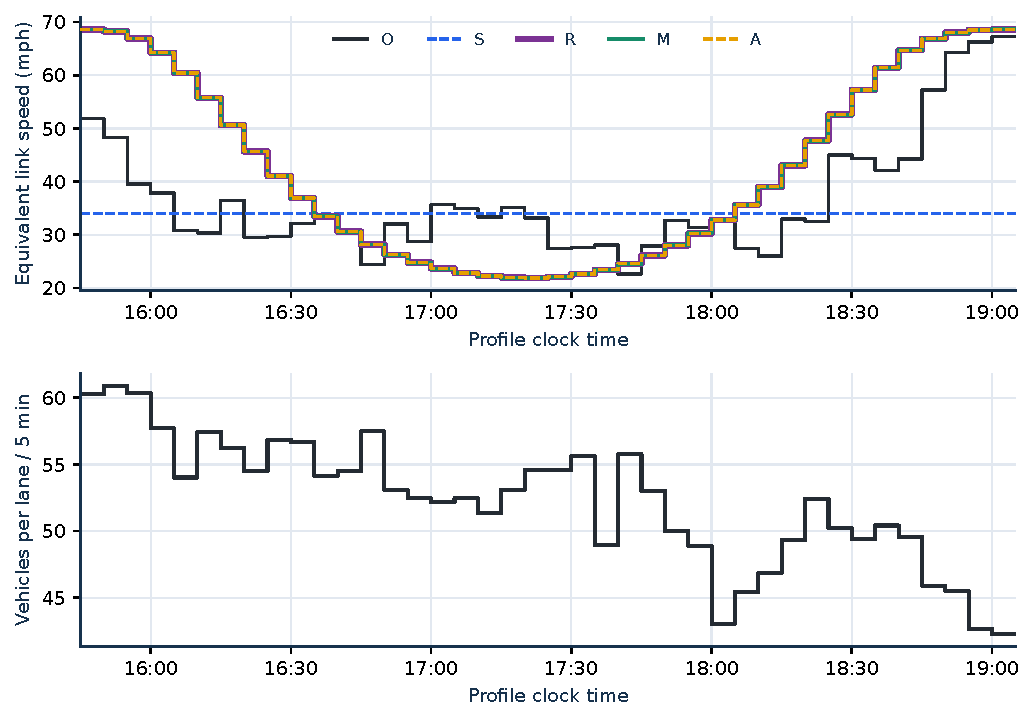
\includegraphics[width=\linewidth]{../../figures/traffic_profiles.pdf}\end{center}
\textbf{Equivalent speed for M/A.} The time allocation gives
\[v_i^{\rm eff}=\frac{v_f\bar t_{f,i}+v_q\bar t_{q,i}}{\bar t_{f,i}+\bar t_{q,i}}=\frac{L}{\bar t_{f,i}+\bar t_{q,i}}.\]
R, M and A overlap because they have identical allocated vehicle-hours and distance. Their operating speeds and rates differ. M/A use $v_f=68.642$ and $v_q=7.882$ mph internally, rather than the displayed equivalent speed.
\notebox{The common clock is a display allocation: modeled vehicle groups are split into the observed five-minute count groups in cumulative-count order. It preserves every method's total. It does not infer when exhaust was physically released on the roadway.}

\newpage
{\fontsize{19}{23}\selectfont\bfseries\color{navy}VSP profiles over the episode}\par
{\color{muted}Same count-aligned clock as the speed profiles; zero acceleration and level road.}\par
\vspace{4pt}Let $z(v)=\operatorname{VSP}_0(v)$ in kW/t and $a_{ij}$ be the model-node count assigned to observed bin $i$. The plotted VSP is weighted by vehicle-hours:
\[
\bar z_{R,i}=\frac{\sum_j a_{ij}T_j z(v_{R,j})}{H_{R,i}},\qquad
\bar z_{M,i}=\bar z_{A,i}=\frac{\sum_j a_{ij}[t_{f,j}z(v_f)+t_{q,j}z(v_q)]}{H_{R,i}}.
\]
O uses $z(v_i)$; S uses the constant $z(\bar v_{\rm obs})$. M and A overlap because their operating speeds and exposure are identical. A changes only the emission-rate approximation.
The supplied mapping is $z(v)=(0.156461s_v+0.00200193s_v^2+0.000492646s_v^3)/1.4788$, with $s_v=0.44704v$ for speed $v$ in mph.
\begin{center}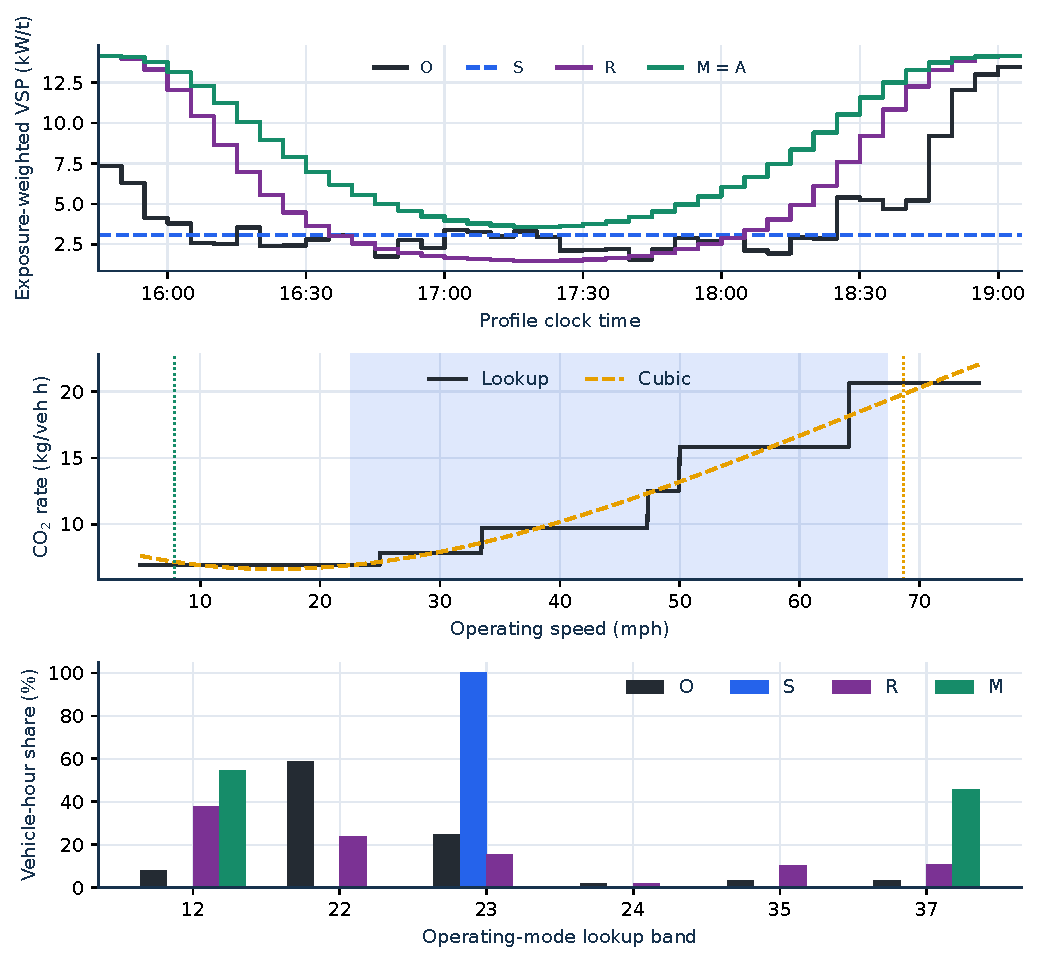
\includegraphics[width=.95\linewidth]{../../figures/vsp_and_rate_mapping.pdf}\end{center}
\textbf{Top: VSP over time.} Each step spans one observed five-minute bin. This exposure-weighted quantity generally differs from $z(v_i^{\rm eff})$, which is supplied separately in the CSV. It is not an emission rate or a measured trajectory VSP.\par
\textbf{Middle: rate assignment.} Shading marks observed speeds; dotted lines mark $v_q$ (green) and $v_f$ (orange). The lookup and cubic functions map the operating conditions to rates.\par
\textbf{Bottom: total exposure by lookup band.} O and R span several bands; S uses one band. M allocates exposure to modes 12 and 37. A uses those same two speeds with cubic rates.
\notebox{Equal equivalent speed does not imply equal operating-state VSP. R, M and A share fitted vehicle-hours, but M/A can place substantial exposure at free-flow speed while compensating with a slow queue state. The VSP profile is a diagnostic average of those states, not a new rate input. The emission calculations and all 20 episode totals are unchanged.}

\newpage
{\fontsize{19}{23}\selectfont\bfseries\color{navy}Rates and five-minute contributions}\par
{\color{muted}Same observed count in each bin; method-specific travel-time exposure and rates.}\par
\begin{center}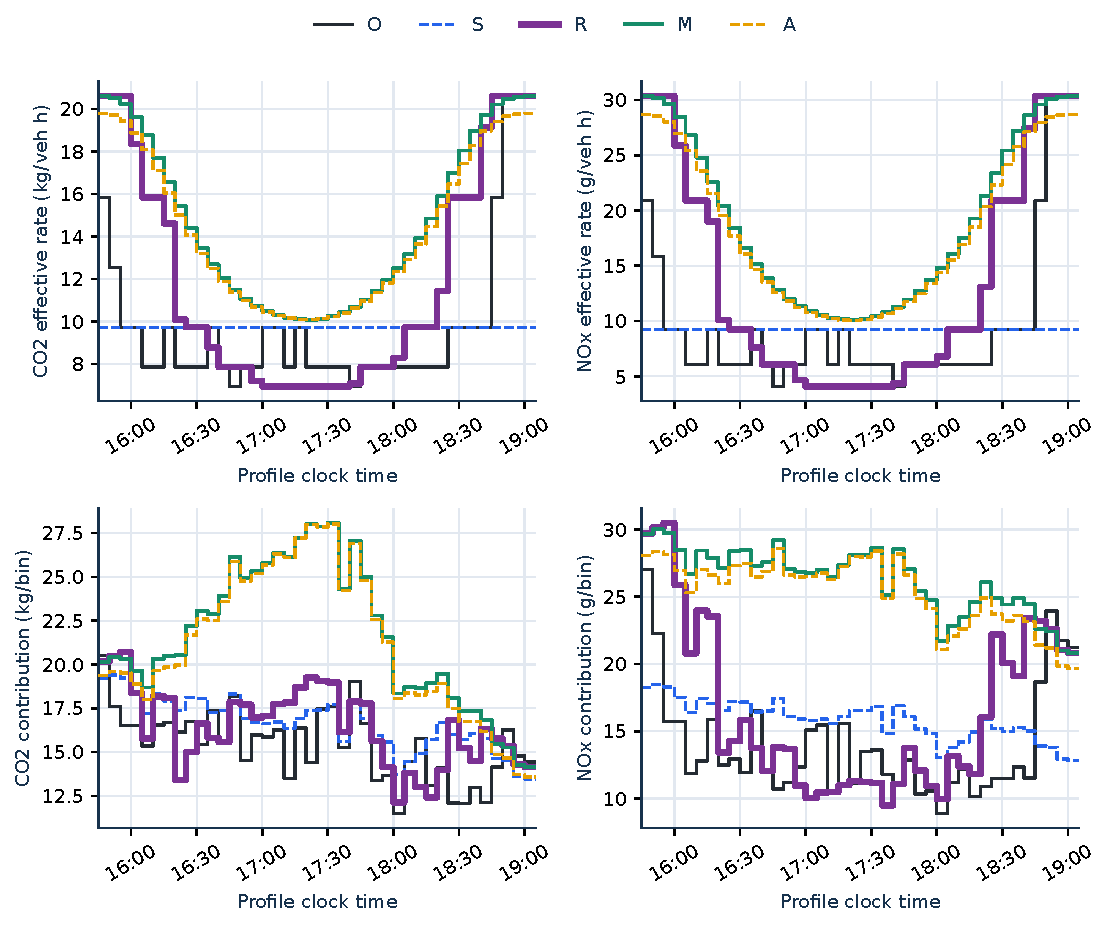
\includegraphics[width=\linewidth]{../../figures/emission_time_series.pdf}\end{center}
\textbf{Top: effective rate.} In each bin, $r^{\rm eff}_{m,i}=E_{m,i}/H_{m,i}$. For R this averages the assigned rates of its reconstructed vehicle groups. For M/A it averages the free-flow and queue rates by their time allocations. It is generally not the lookup at the displayed equivalent speed.
\par\vspace{8pt}\textbf{Bottom: contribution from that bin's vehicles.} $E_{m,i}=H_{m,i}r^{\rm eff}_{m,i}$. The five-minute duration creates the vehicle count; a vehicle's exposure is its complete-link travel time. Each plotted series sums to the corresponding episode total on page 2.
\notebox{O and S have identical total exposure. Their five-minute contributions differ because S assigns one constant trip time and rate to every counted vehicle. R/M/A share fitted exposure; their remaining differences come from the speeds at which rates are evaluated and from lookup versus cubic approximation.}

\newpage
{\fontsize{19}{23}\selectfont\bfseries\color{navy}How the contributions accumulate}\par
{\color{muted}Vehicle-order view on the left; conservative common-clock allocation on the right.}\par
\begin{center}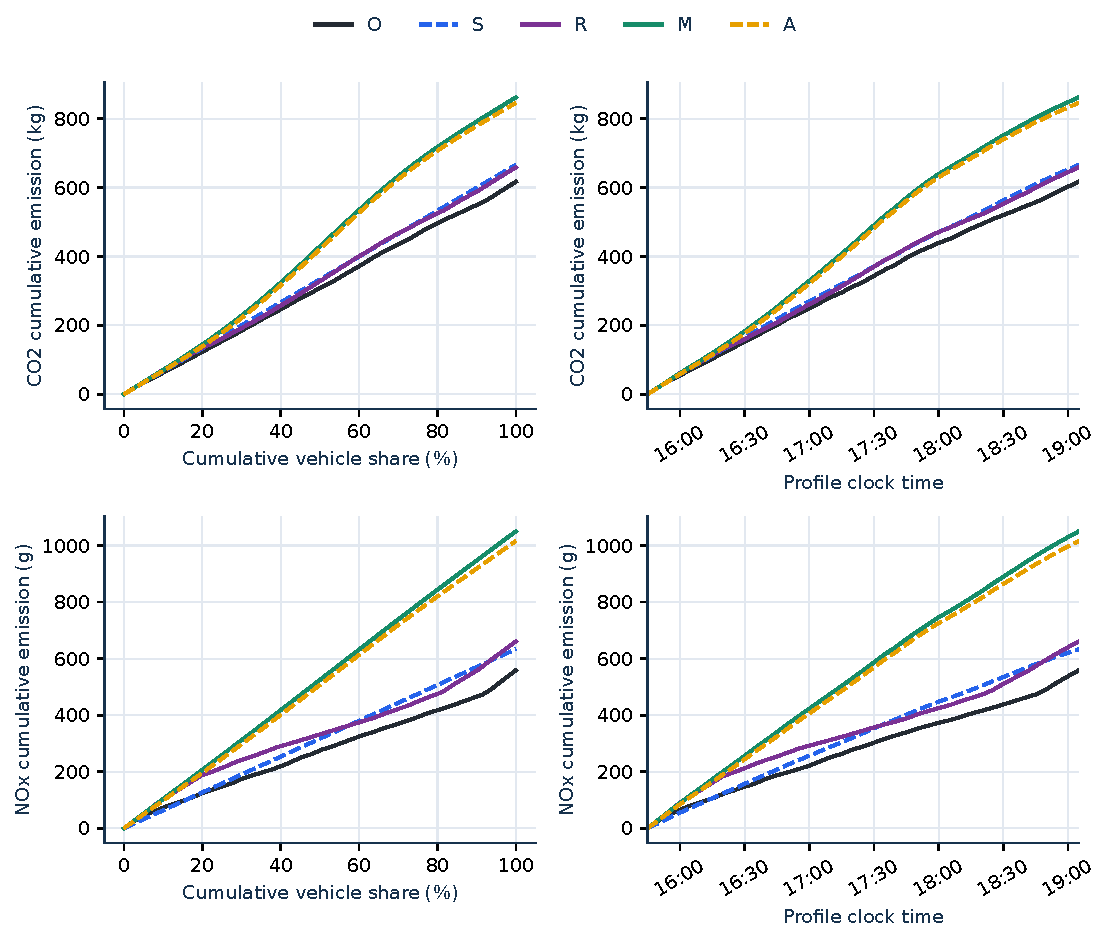
\includegraphics[width=\linewidth]{../../figures/cumulative_contributions.pdf}\end{center}
\textbf{Vehicle share.} O follows the observed bin order. R/M/A follow reconstructed entry-group order. S has constant emission per vehicle. All curves terminate at the same count $D$, with their own episode emission total.
\par\vspace{8pt}\textbf{Clock time.} Each boundary value sums the complete-link emissions assigned to all preceding bins. Connecting lines interpolate bin contributions for display and imply no sub-bin exhaust timing.
\notebox{For observed cumulative counts $B_i$ and modeled cumulative counts $N_j$, the overlap count is
\[n_{ij}=\max\{0,\min(B_i,N_j)-\max(B_{i-1},N_{j-1})\}.\]
Use $H_i=\sum_jn_{ij}T_j$ and $E_i=\sum_jn_{ij}e_j$. Both count and emission totals are conserved. The underlying 384-node integration and all 40 common-clock rows are supplied as CSV files.}

\newpage
{\fontsize{19}{23}\selectfont\bfseries\color{navy}Where the differences enter}\par
{\color{muted}An exact signed accounting sequence, conditional on the chosen order.}\par
Define $E_{S,p}=H_{\rm pred}r_0(DL/H_{\rm pred})$, a single-speed calculation with the fitted exposure shared by R/M/A. Then
\[
E_A-E_O=(E_S-E_O)+(E_{S,p}-E_S)+(E_R-E_{S,p})+(E_M-E_R)+(E_A-E_M).
\]
\begin{center}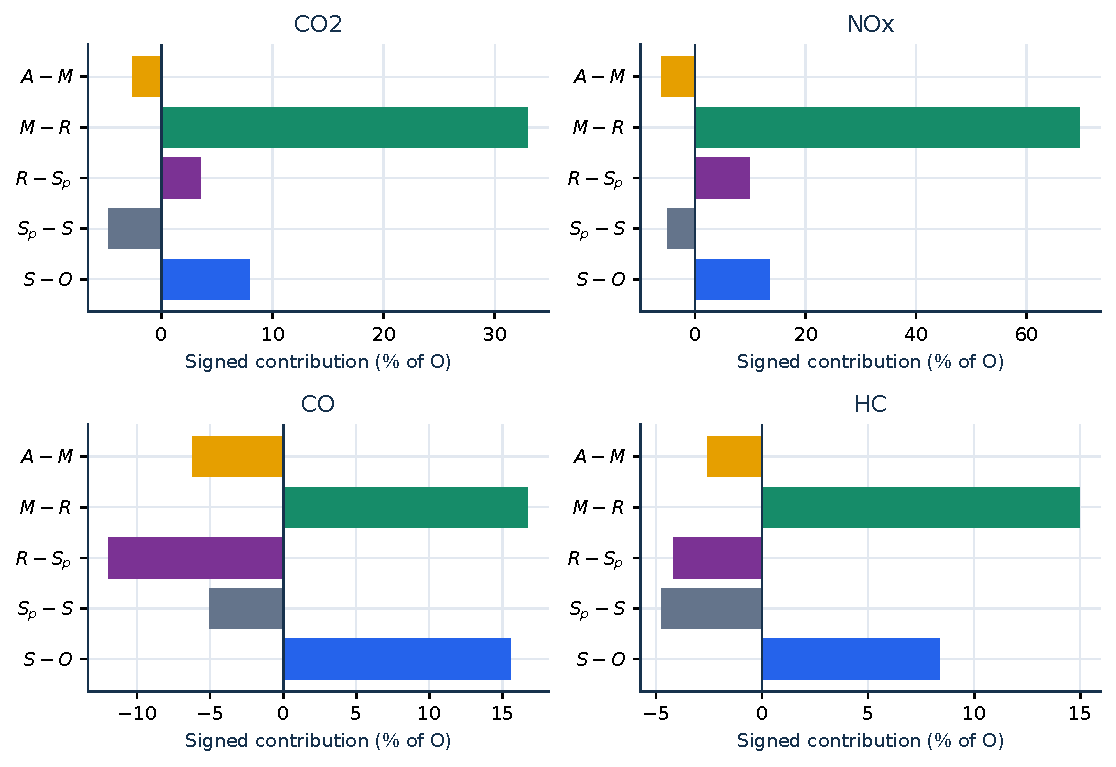
\includegraphics[width=.96\linewidth]{../../figures/error_components.pdf}\end{center}
\textbf{Signed components as a percentage of O}\par
\par\noindent\begin{tabular*}{\linewidth}{@{\extracolsep{\fill}}lrrrrr@{}}\toprule
Pollutant & S$-$O & S$_p-$S & R$-$S$_p$ & M$-$R & A$-$M\\\midrule
CO$_2$ & +7.97 & -4.73 & +3.54 & +32.95 & -2.57\\\midrule[.3pt]
NO$_x$ & +13.40 & -4.97 & +9.86 & +69.68 & -6.13\\\midrule[.3pt]
CO & +15.54 & -5.06 & -11.93 & +16.71 & -6.20\\\midrule[.3pt]
HC & +8.35 & -4.75 & -4.18 & +14.98 & -2.56\\\bottomrule\end{tabular*}\par
\vspace{7pt}The fitted exposure differs from O by -4.382\%. $S_p-S$ combines this exposure change with any lookup-rate change caused by the fitted mean speed. $R-S_p$ adds reconstructed trip-speed variation. $M-R$ changes the operating-speed representation at equal fitted vehicle-hours. $A-M$ changes only the rate approximation.
\notebox{The traffic screens pass, so a large travel-time calibration error is not needed to create this discrepancy. M and R have the same fitted vehicle-hours, but evaluate rates at different speed distributions. The large M--R component isolates that representation difference within this accounting sequence. It does not identify the unknown real trajectory emissions.}
\vspace{7pt}\textbf{Audit and source files.} All 20 episode totals reproduce the frozen matched-episode record. The supplied selection table contains all 137 cases, the five traffic error screens, the physical check and the four passing cases. The full-precision inputs, rate-band exposure, common-clock data, error components, editable vector figures and this report source are included with the case. No calibration, episode boundary or published result was replaced.
\end{document}
